\documentclass[polish,polish,a4paper]{article}
\usepackage[utf8]{inputenc}
\usepackage[T1]{fontenc}
\usepackage[polish]{babel}
\usepackage{anysize}
\usepackage{siunitx}
\usepackage{graphicx}
\usepackage{listings}
\usepackage{pgfplots}
\usepackage{xcolor} % do komentarzy
\usepackage{diagbox} % macierz pomyłek
\usepackage{color, colortbl}
\usepackage{caption}

\definecolor{Gray}{gray}{0.9}

\marginsize{2cm}{2cm}{2cm}{2cm}

\title{Wykrywanie naczyń dna siatkówki oka}
\author{Przemysław Ambroży (141182), Błażej Celmer (141197)}

\begin{document} 
	\maketitle
	
	\section{Wstęp}
		Ćwiczenie zakłada wykrycie oraz zaznaczenie naczyń na zdjęciach dna oka. 
		Skorzystamy z technik przetwarzania obrazu, uczenia maszynowego oraz głębokiej sieci neuronowej.
		Wyniki tych trzech metod porównamy ze sobą za pomocą wizualnej reprezentacji oraz miar jakości.
		
	\section{Środowisko i dane}
		Skorzystaliśmy z języka Python w środowisku Jupyter Notebook,
		co pozwoliło uzyskać interfejs użytkownika niskim kosztem.
		Skorzystaliśmy również z bibliotek, które oferowały dodatkowe funkcjonalności, m.in.:
		
		\begin{description}
			\item[skimage] przetwarzanie obrazów
			\item [sklearn] klasyfikator -- drzewo decyzyjne
			\item [keras] sieci neuronowe 
			\item [pickle] zapis oraz odczyt wytrenowanych klasyfikatorów
		\end{description}
		
		Jako dane wykorzystaliśmy zbiór CHASE, zawierający obrazy dna siatkówki oczu (lewych i prawych),
		a~także maski z naczyniami oznaczonymi przez lekarzy. 
		Dane pochodzą ze strony \\ \texttt{https://blogs.kingston.ac.uk/retinal/chasedb1/}
		
	\section{Opis metod}
		\subsection{Przetwarzanie obrazu}
		
		W tej metodzie obraz został poddany podstawowym operacjom:
			\begin{enumerate}
				\item skala szarości -- 
					skupiamy się jedynie na jasności obrazu
					
				\item dostosowanie gamma
				
				\item dostosowanie ekspozycji
				
				\item rozmycie --
					rozmycie gaussowskie  powinno zmniejszyć szum, który uwydatniłby się po wyostrzeniu
				
				\item wyostrzenie --
					uwydatnia granice naczyń
					
				\item wykrywanie krawędzi --
					uwydatnia granice naczyń, algorytm Frangi
					
				\item maska binarna -- 
					funkcja ustalająca poziom odcięcia, 
					dzięki któremu wyznaczamy klasyfikację binarną
					
				\item otwarcie -- 
					funkcja wykonująca operacje erozji oraz dylatacji, 
					pozwala zmniejszyć szum
					
				\item usunięcie okręgu -- 
					powyższe operacje wygenerują jasny okrąg dookoła oka. Ta operacja zniweluje ten efekt poprzez nadpisanie.
			\end{enumerate}
			
		\begin{figure}[!h]
			\centering
			\begin{minipage}{0.3\linewidth}
				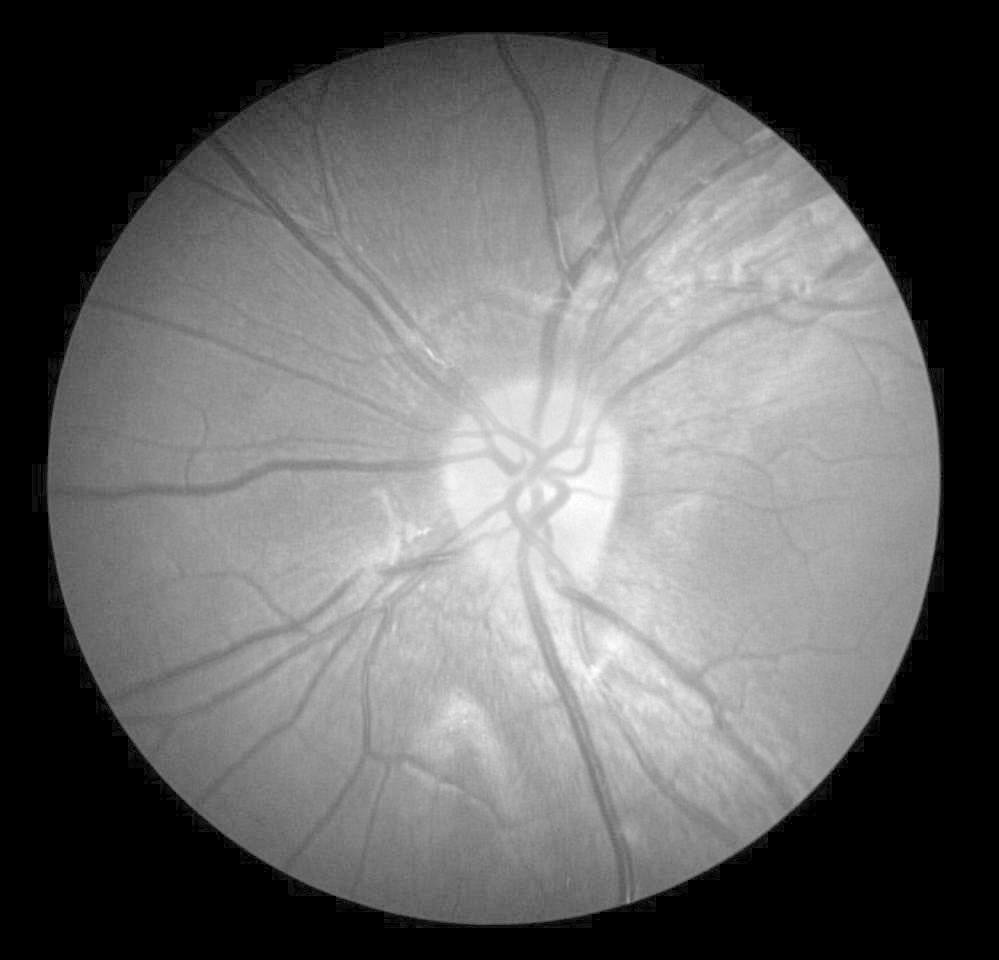
\includegraphics[width=\linewidth]{./dane/metoda1/gamma.png}
				\caption*{Korekta gamma}
			\end{minipage}
			\begin{minipage}{0.3\linewidth}
				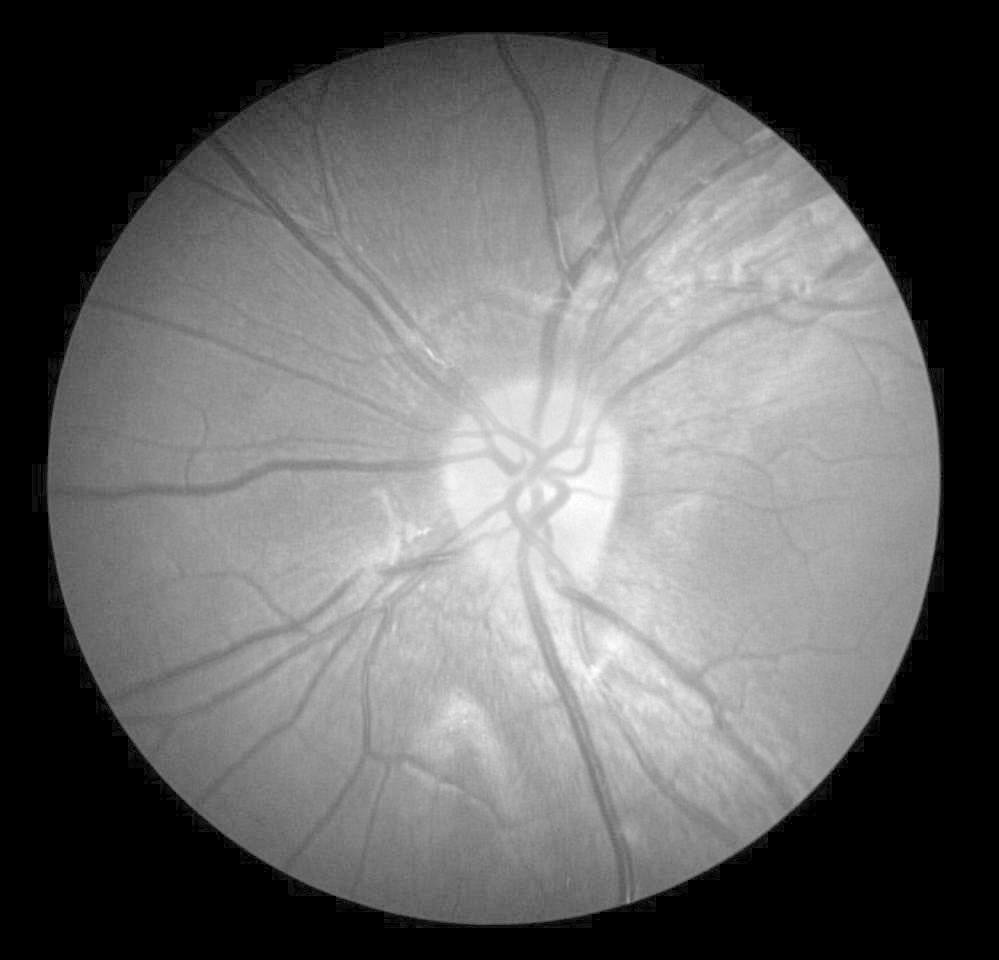
\includegraphics[width=\linewidth]{./dane/metoda1/exposure.png}
				\caption*{Korekta ekspozycji}
			\end{minipage}
			\begin{minipage}{0.3\linewidth}
				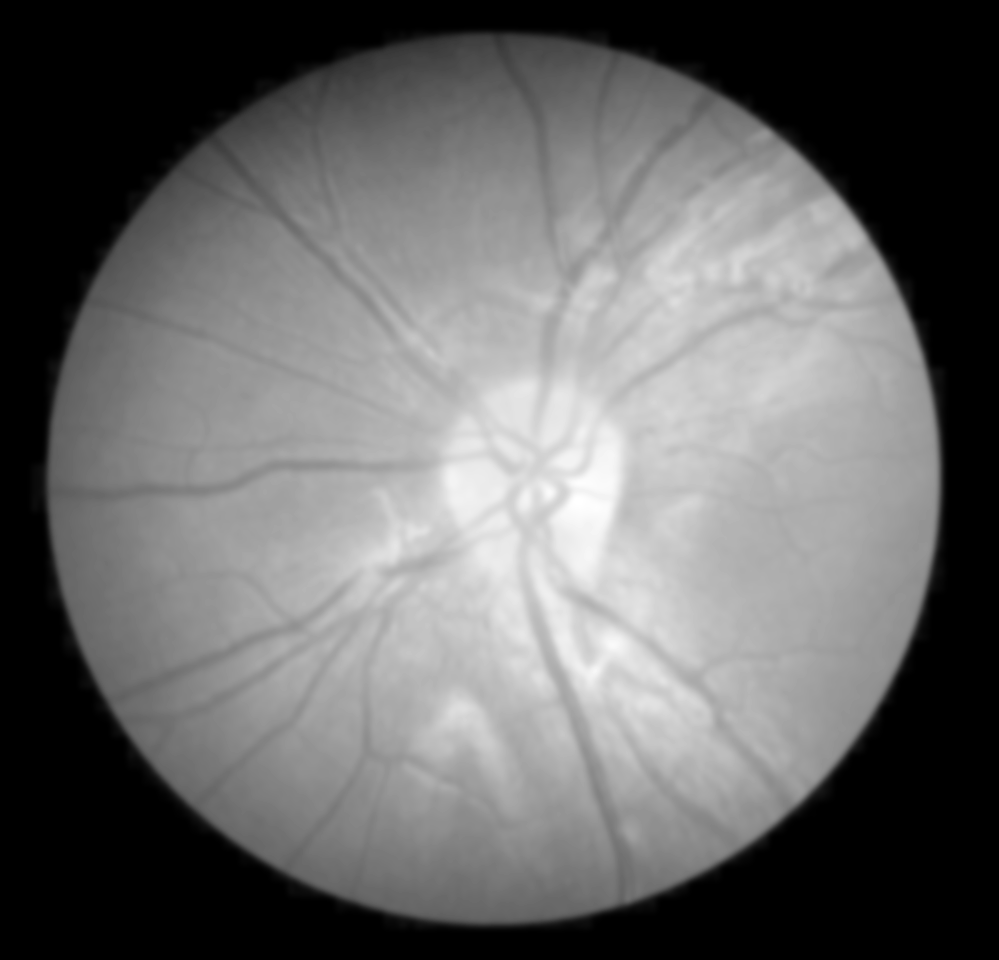
\includegraphics[width=\linewidth]{./dane/metoda1/blur.png}
				\caption*{Rozmycie}
			\end{minipage}
			\begin{minipage}{0.3\linewidth}
				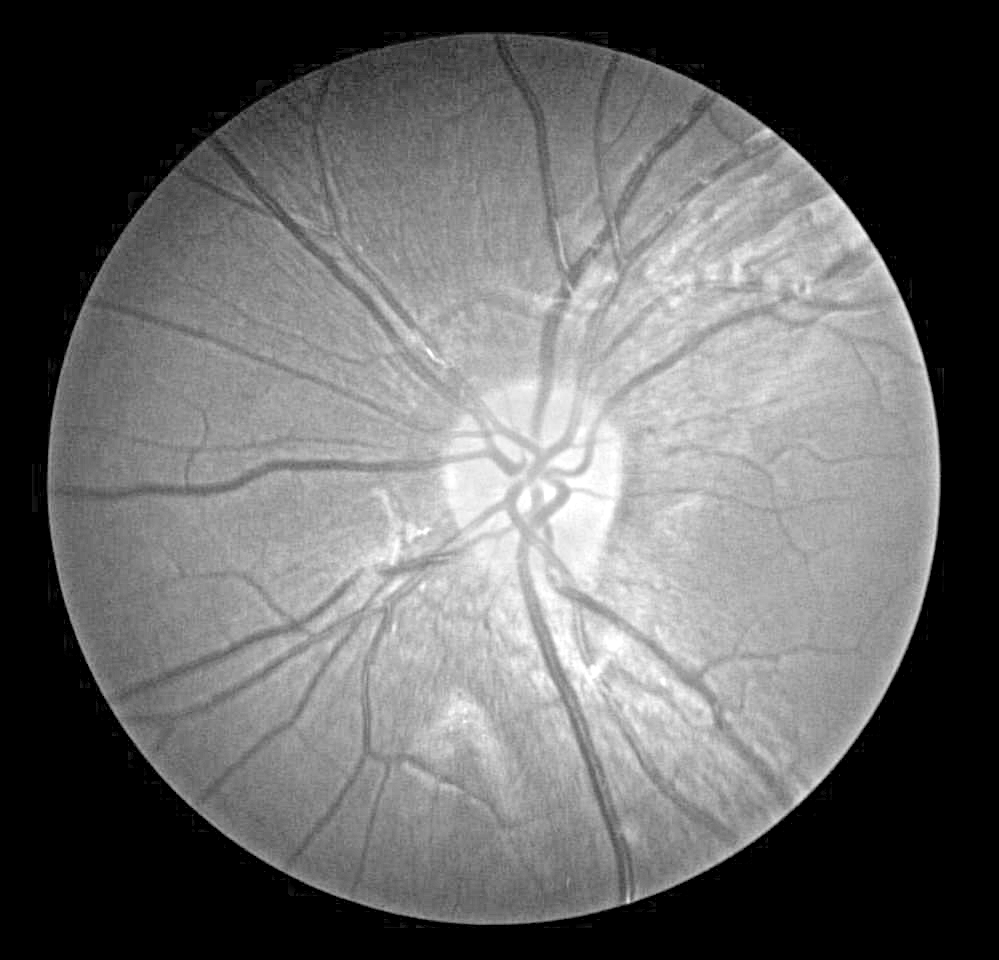
\includegraphics[width=\linewidth]{./dane/metoda1/sharpen.png}
				\caption*{Wyostrzenie}
			\end{minipage}
			\begin{minipage}{0.3\linewidth}
				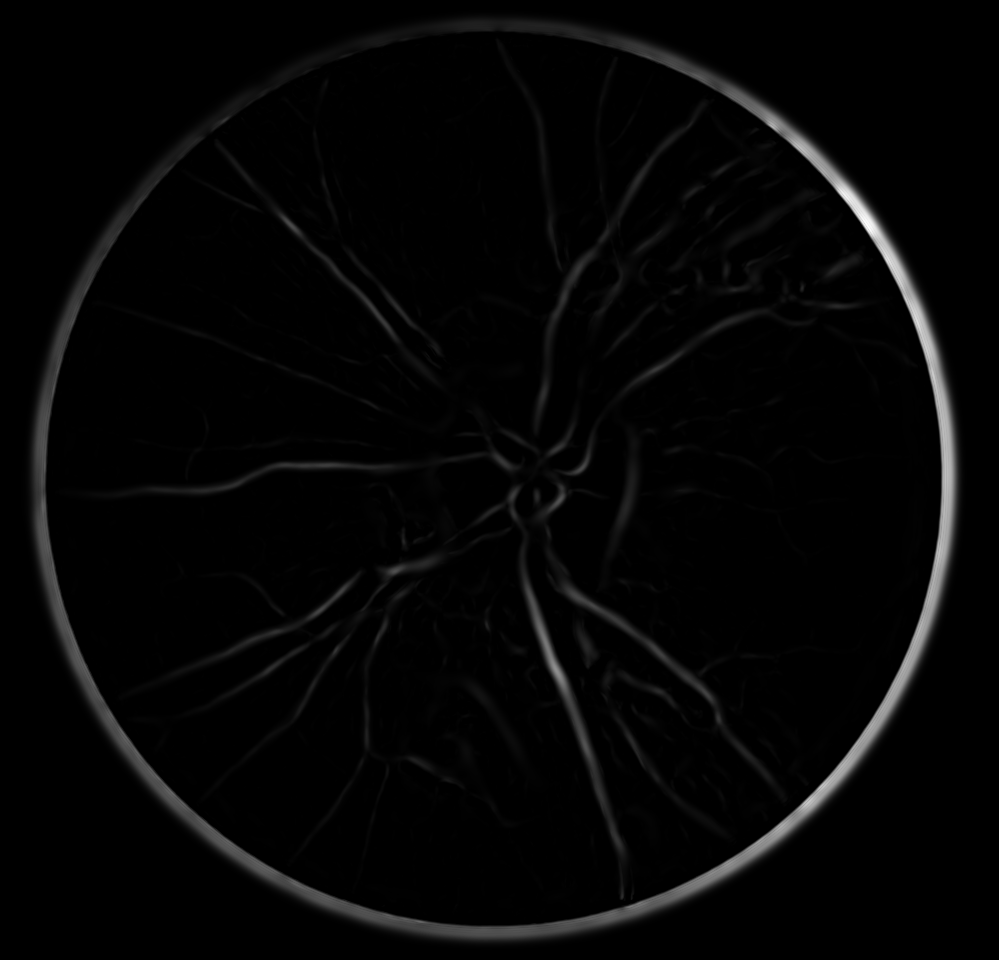
\includegraphics[width=\linewidth]{./dane/metoda1/edges.png}
				\caption*{Krawędzie}
			\end{minipage}
			\begin{minipage}{0.3\linewidth}
				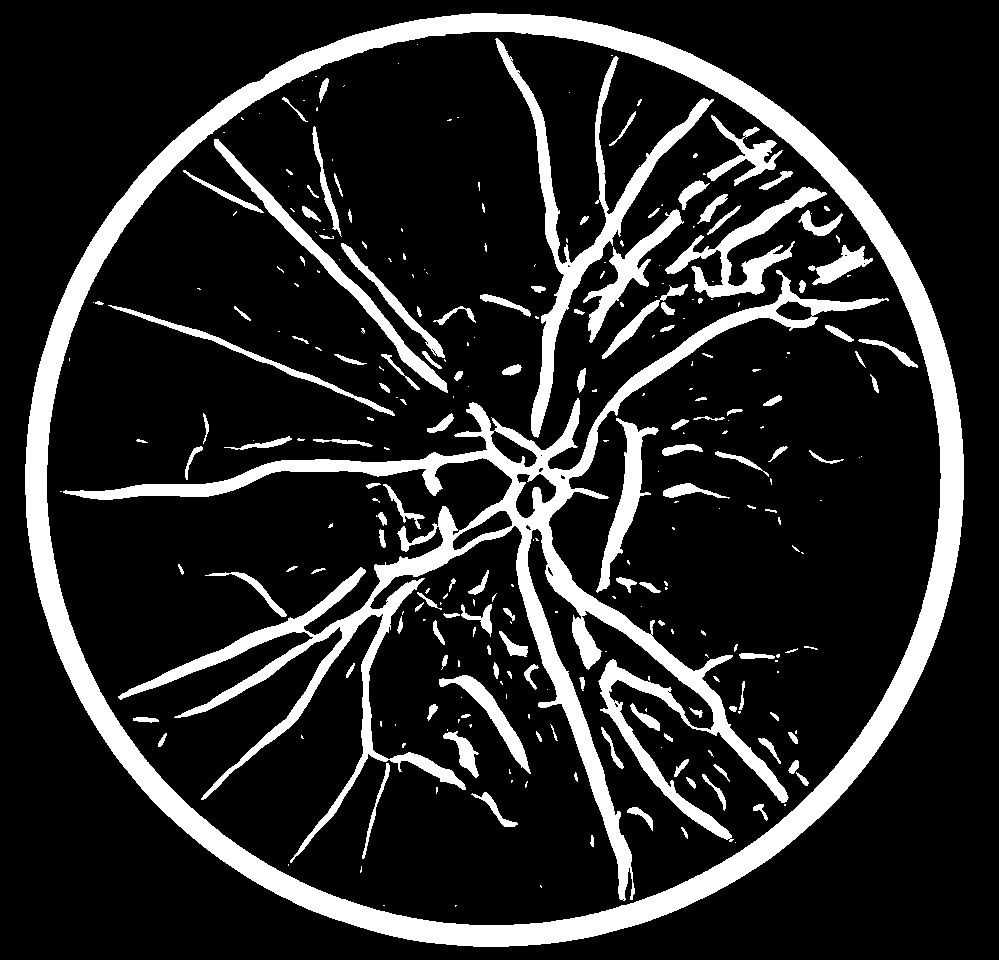
\includegraphics[width=\linewidth]{./dane/metoda1/binary.png}
				\caption*{Maska binarna}
			\end{minipage}
			\begin{minipage}{0.3\linewidth}
				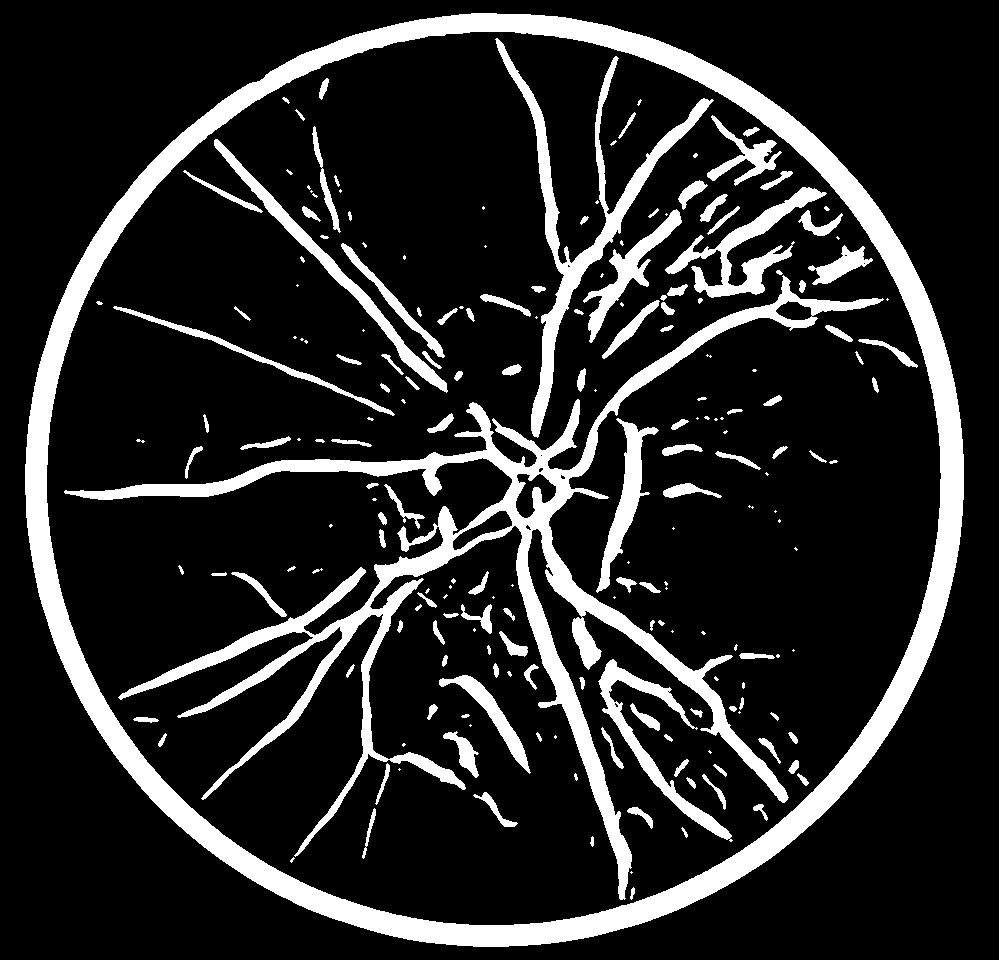
\includegraphics[width=\linewidth]{./dane/metoda1/opening.png}
				\caption*{Otwarcie}
			\end{minipage}
			\begin{minipage}{0.3\linewidth}
				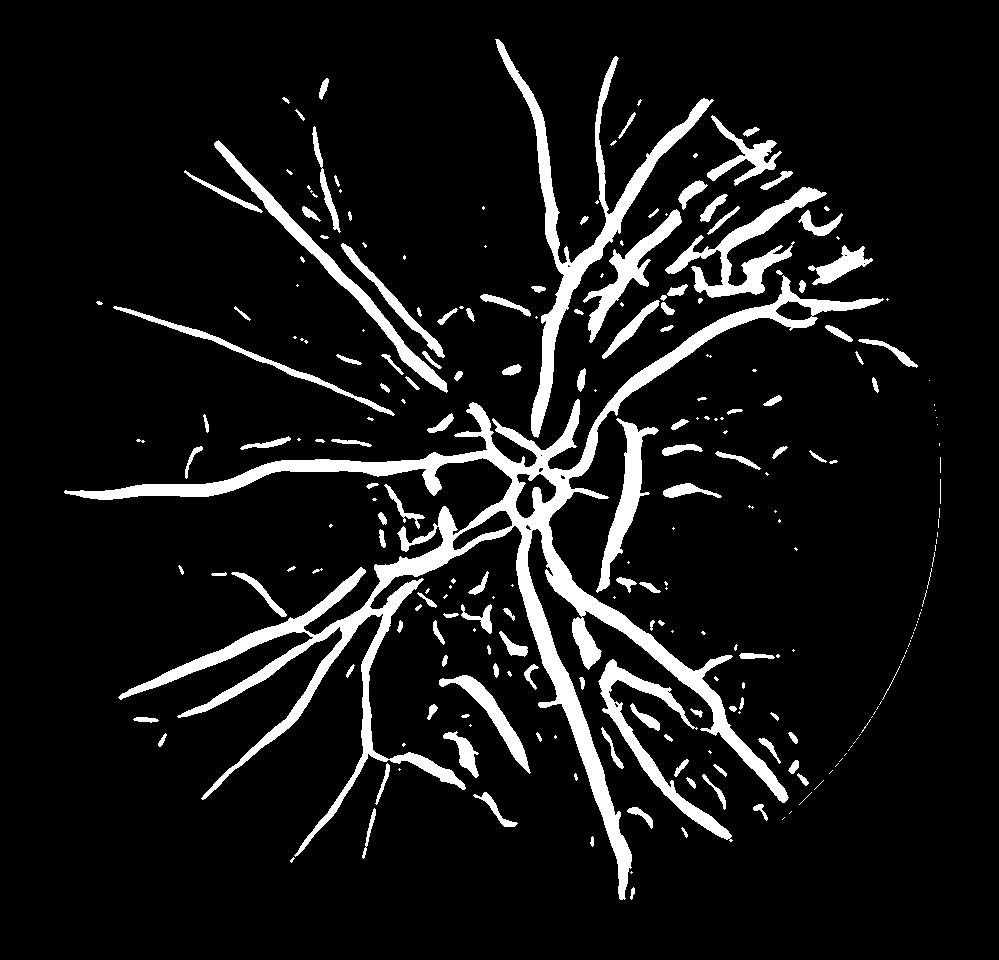
\includegraphics[width=\linewidth]{./dane/metoda1/ring.png}
				\caption*{Usunięcie okręgu}
			\end{minipage}
			\caption*{Etapy przetwarzania obrazu}
		\end{figure}
		
		\subsection{Uczenie maszynowe}
			Na początek wstępnie edytujemy obraz wejściowy. Używamy niektórych funkcji z przetwarzania obrazu tj.:
			\begin{itemize}
				\item dostosowanie gamma
				\item dostosowanie ekspozycji
				\item rozmycie gaussowskie
				\item wyostrzenie
			\end{itemize}
			W kolejnym kroku dzielimy obraz na fragmenty o określonym rozmiarze (zazwyczaj od 5x5 do 9x9 pikseli).
			Te fragmenty zachodzą na siebie, tak każdy piksel ze zdjęcia posiadał fragment, w którym on jest na środku.
			Z pobranych fragmentów usuwamy te, które są poza obszarem oka (czarne tło).
			Następnie wybieramy losowe próbki ze zdjęcia w proporcji 50\% z klasy negatywnej i 50\% z pozytywnej.
			Każdą próbkę zamieniamy na zestaw cech dla klasyfikatora.
			W naszym przypadku jest to wektor wartości RGB kolejnych pikseli we fragmencie. 
			Proces jest powtarzany dla kilku zdjęć, aby otrzymać więcej danych.
			
			Uczymy klasyfikator, korzystając z wygenerowanych cech wraz z odpowiadającym im wynikiem z maski eksperckiej. 
			Nasz klasyfikator to drzewo decyzyjne (\texttt{sklearn.tree.DecisionTreeClassifier}).
			Został wytrenowany na zbiorze 500 tysięcy losowych próbek o rozmiarze 9x9 ze zdjęć 
			\textit{01L}, \textit{01R}, \textit{02R}, \textit{03L}, \textit{03R}.
		
		\subsection{Głęboka sieć neuronowa}
		
			Obraz, przed wejściem do sieci, dzielony jest na fragmenty o wielkości 19x19 pikseli.
Następnie na każdym fragmencie wykonywana jest globalna normalizacja kontrastu.
Obliczane są średnia i odchylenie standardowe każdego kanału we fragmencie (czerwony, zielony i niebieski).
Następnie każdy kanał każdego piksela jest normalizowany -- odejmowana
jest od niego średnia i dzielony jest przez odchylenie standardowe.
Poniżej przedstawione zostało działanie tej funkcji na wybranym fragmencie:
\begin{figure}[!h]
	\centering
	\begin{minipage}{0.3\linewidth}
		
\includegraphics[scale=0.5]{./dane/preprocess.png}
	\end{minipage}
	\begin{minipage}{0.3\linewidth}
		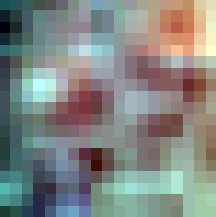
\includegraphics[scale=0.5]{./dane/postprocess.png}
	\end{minipage}
\end{figure}
\\ Do trenowania wykorzystano 500 tysięcy losowych fragmentów pochodzących z plików \textit{01L}, \textit{01R}, \textit{02L}, \textit{02R}, \textit{03L}, \textit{03R}. Dane zostały następnie podzielone na zbiór treningowy (67\%) i testowy (33\%).

Sieć została stworzona z wykorzystaniem biblioteki \texttt{keras}.
Składa się z 23 warstw i przypomina architekturę U-Net. 
Początkowo zastosowano dwie warstwy konwolucyjne o filtrze (wymiarowości wyjścia) równym 32 i~rozmiarze okna 3x3.
Następnie zastosowano warstwę max pooling o oknie 2x2 przemieszczającym się o 2, która zmniejsza wielkość wyjścia.
Taki zestaw warstw powtórzono, zmieniając filtr na wartości: 48, 64, 96, 64, 38, 32.
Na końcu zastosowano warstwę wypłaszczającą oraz warstwę, gdzie każdy neuron jest połączony ze sobą (Dense) o sigmoidalnej funkcji aktywacji.
Do danych z wyjścia sieci zastosowano próg 0.3, powyżej którego piksel uznawany jest za naczynie.
Wstępna ocena sieci na danych testowych:
\begin{itemize}
    \item strata (loss) = 8.39%
    \item trafność (accuracy) = 96.99%
\end{itemize}

\subsubsection*{Rozmiar wycinka}
Zastosowano rozmiar wycinka 19x19. Mniejsze wycinki powodowały pogorszenie parametrów, przy większych czas tworzenia fragmentów i wstępnego przetwarzania był zbyt długi. Poniżej porównanie miar dla tego samego obrazka przy zastosowaniu różnych wycinków:
\begin{center}
\begin{tabular}{|>{\columncolor[gray]{0.9}}r|c|c|}
\hline \rowcolor{Gray}
\textbf{Rozmiar wycinka} & \textbf{17} & \textbf{19}  \\ \hline \hline
TP                & 59039                                         & 58529                                         \\ \hline
TN                & 829336                                        & 830092                                        \\ \hline
FP                & 23448                                         & 18842                                         \\ \hline
FN                & 16129                                         & 16639                                         \\ \hline
accuracy          & 0.9574                                        & 0.9616                                        \\ \hline
sensitivity       & 0.7854                                        & 0.7786                                        \\ \hline
specificity       & 0.9725                                        & 0.9778                                        \\ \hline
balanced accuracy & 0.879                                         & 0.8782                                        \\ \hline
F1                & 0.749                                         & 0.7674                                        \\ \hline
Obraz             & 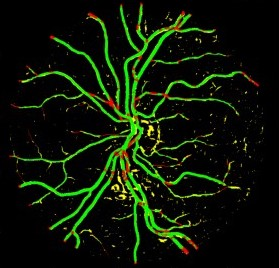
\includegraphics[width=5cm]{./dane/box17.jpg} & 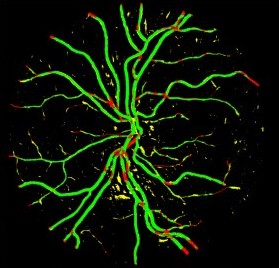
\includegraphics[width=5cm]{./dane/box19.jpg} \\ \hline
\end{tabular}
\end{center}
		
	\section{Wyniki}
		Obrazy wynikowe dla poszczególnych metod są przedstawione jako porównanie z maską ekspercką.
		\begin{description}
			\item [zielony] prawdziwie pozytywna
			\item [żółty] fałszywie pozytywna
			\item [czerwony] fałszywie negatywna
			\item [czarny] prawdziwie negatywna
		\end{description}
\newpage
	
		\subsection{Zdjęcie \textit{04L}}

\begin{figure}[!h]
	\centering
	\begin{minipage}{0.26\linewidth}
		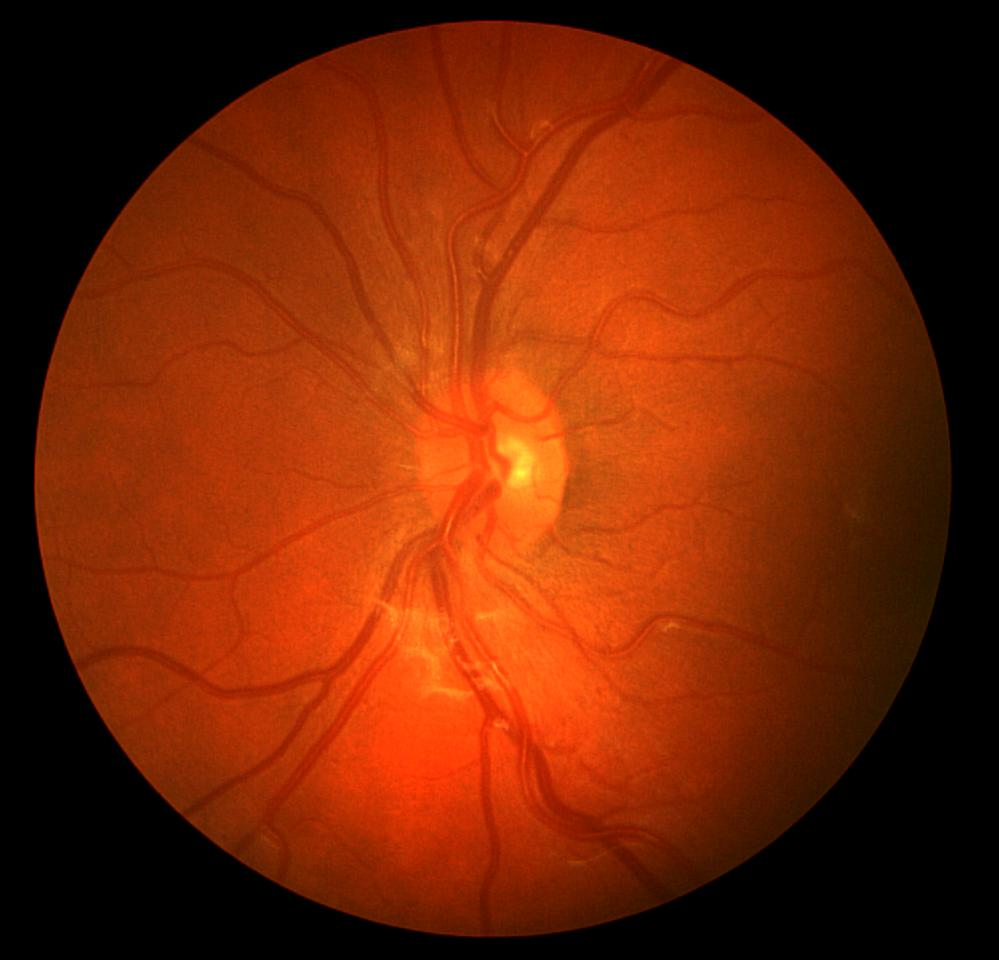
\includegraphics[width=\linewidth]{../chase/Image_04L.jpg}
		\centering
			\small{obraz wejściowy}
	\end{minipage}
	\hfill
	\begin{minipage}{0.26\linewidth}
		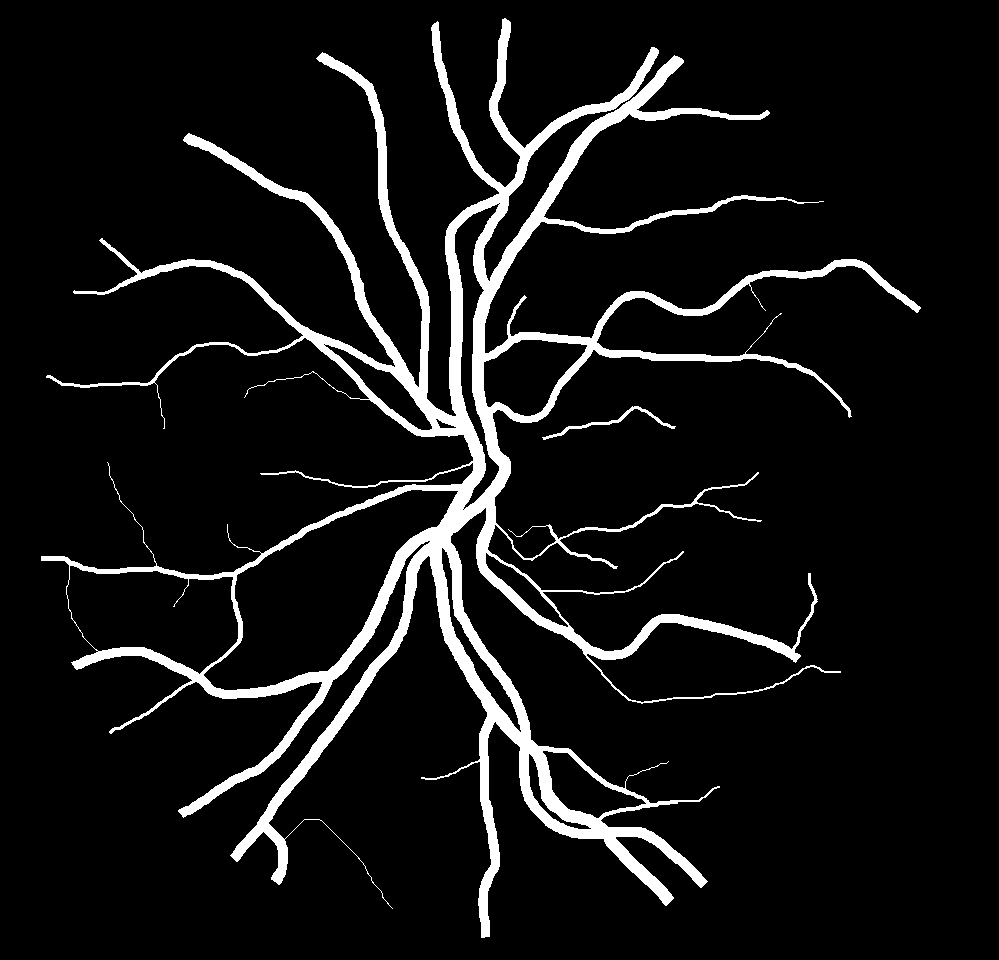
\includegraphics[width=\linewidth]{../chase/Image_04L_1stHO.png}
		\centering
			\small{maska ekspercka}
	\end{minipage}
\end{figure}
\input{./dane/przetwarzanie obrazu/04L.txt}
\input{./dane/uczenie maszynowe/04L.txt}
\input{./dane/głęboka sieć neuronowa/04L.txt}



		\subsection{Zdjęcie \textit{05R}}

\begin{figure}[!h]
	\centering
	\begin{minipage}{0.26\linewidth}
		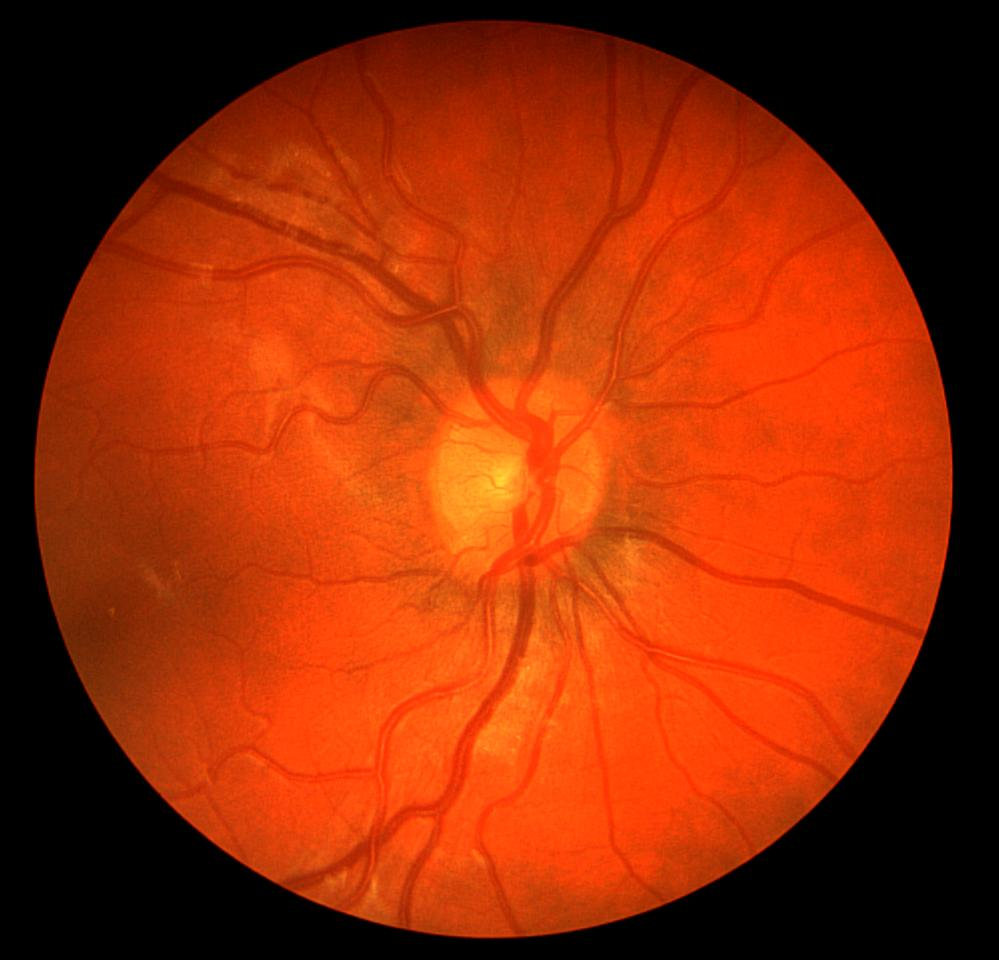
\includegraphics[width=\linewidth]{../chase/Image_05R.jpg}
		\centering
			\small{obraz wejściowy}
	\end{minipage}
	\hfill
	\begin{minipage}{0.26\linewidth}
		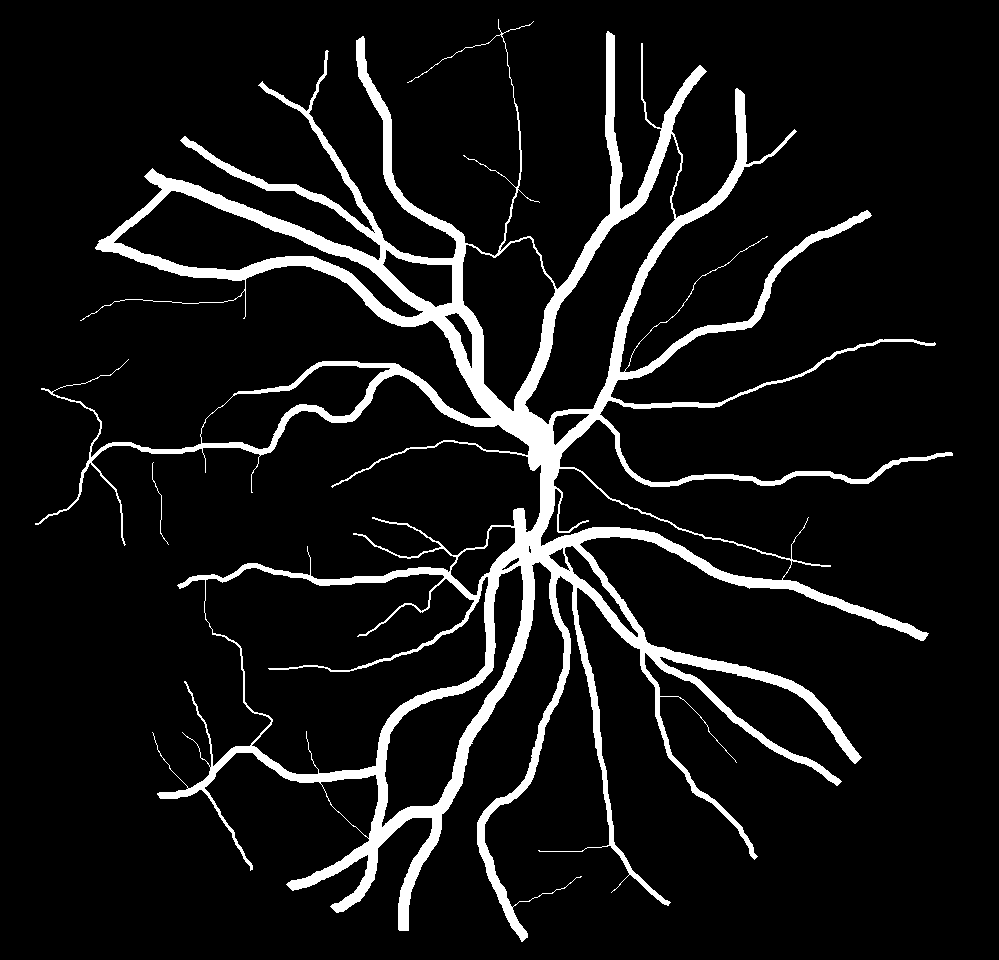
\includegraphics[width=\linewidth]{../chase/Image_05R_1stHO.png}
		\centering
			\small{maska ekspercka}
	\end{minipage}
\end{figure}

\input{./dane/przetwarzanie obrazu/05R.txt}
\input{./dane/uczenie maszynowe/05R.txt}
\input{./dane/głęboka sieć neuronowa/05R.txt}



		\subsection{Zdjęcie \textit{06L}}

\begin{figure}[!h]
	\centering
	\begin{minipage}{0.26\linewidth}
		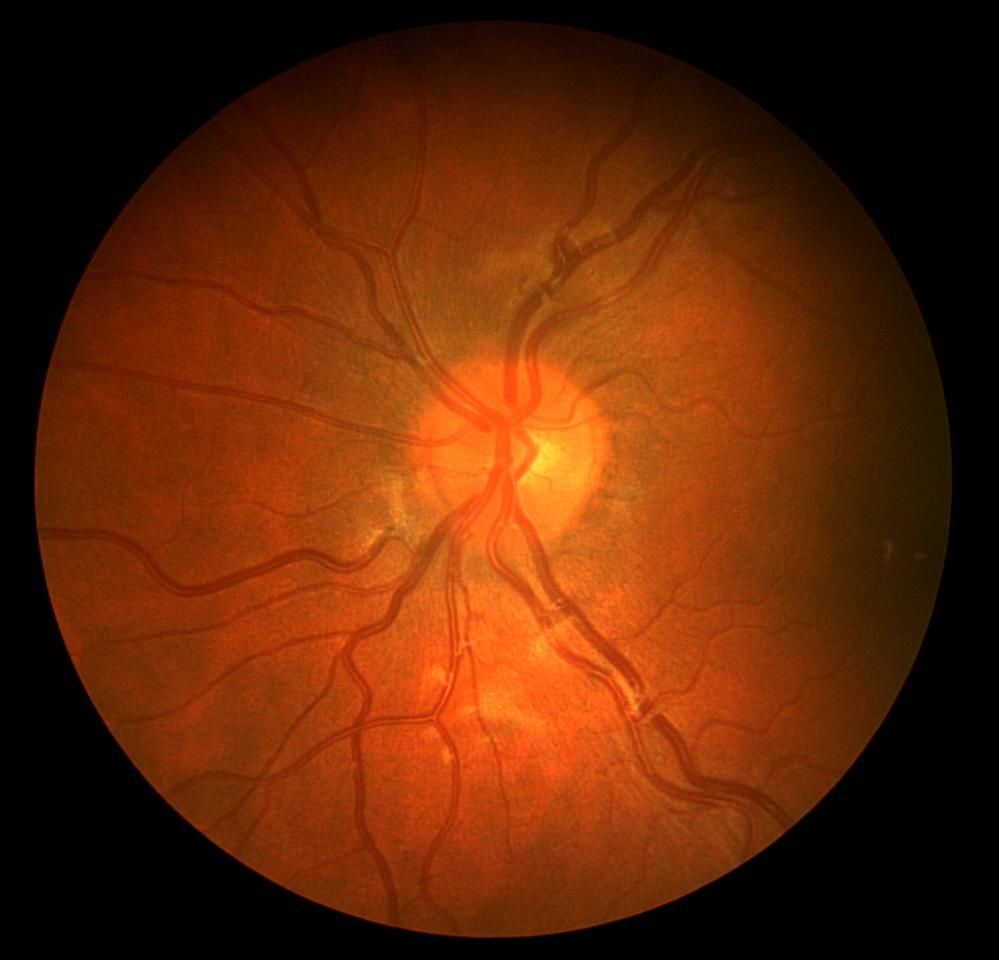
\includegraphics[width=\linewidth]{../chase/Image_06L.jpg}
		\centering
			\small{obraz wejściowy}
	\end{minipage}
	\hfill
	\begin{minipage}{0.26\linewidth}
		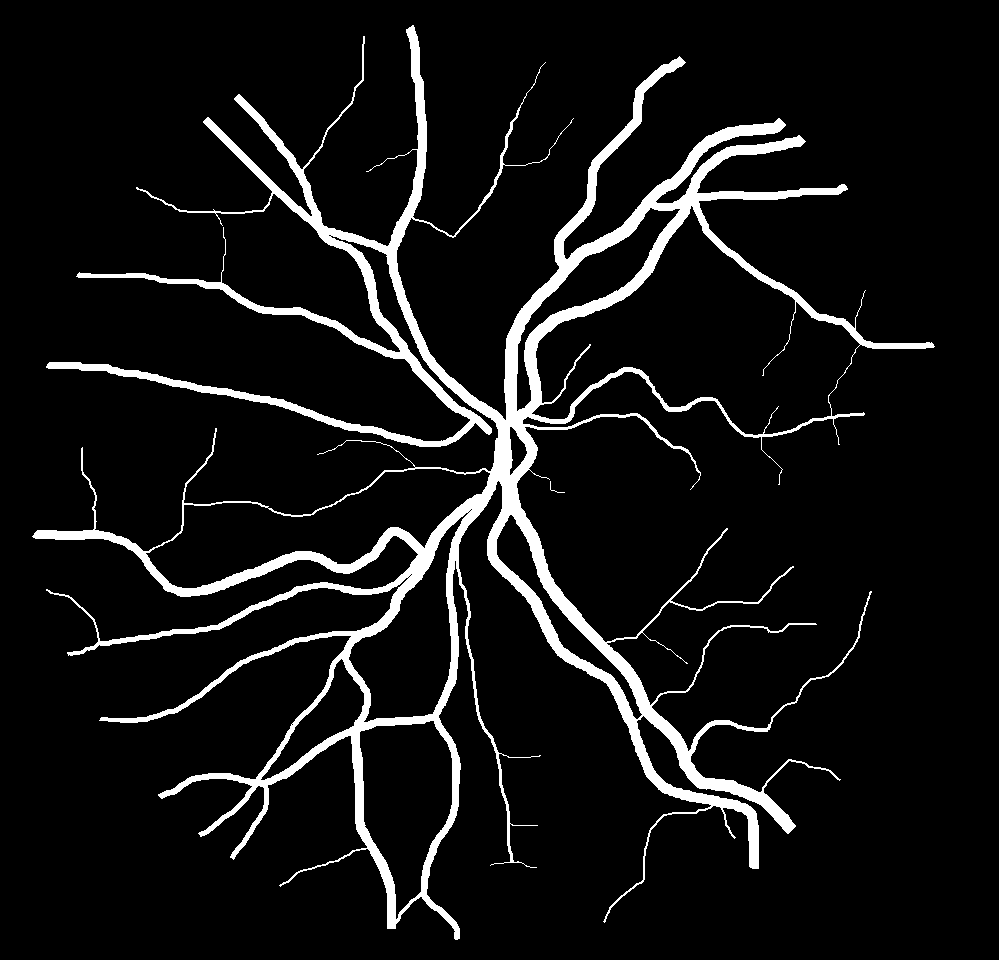
\includegraphics[width=\linewidth]{../chase/Image_06L_1stHO.png}
		\centering
			\small{maska ekspercka}
	\end{minipage}
\end{figure}
\input{./dane/przetwarzanie obrazu/06L.txt}
\input{./dane/uczenie maszynowe/06L.txt}
\input{./dane/głęboka sieć neuronowa/06L.txt}



		\subsection{Zdjęcie \textit{07R}}
		
\begin{figure}[!h]
	\centering
	\begin{minipage}{0.26\linewidth}
		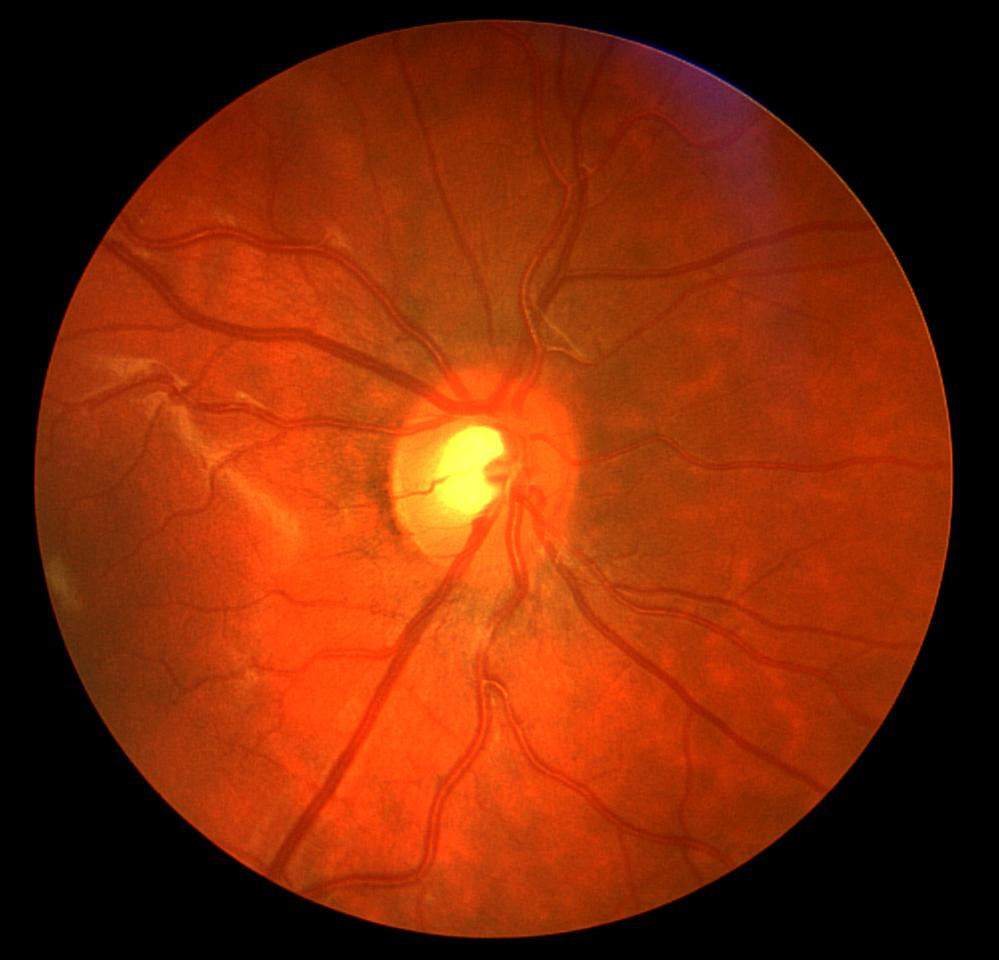
\includegraphics[width=\linewidth]{../chase/Image_07R.jpg}
		\centering
			\small{obraz wejściowy}
	\end{minipage}
	\hfill
	\begin{minipage}{0.26\linewidth}
		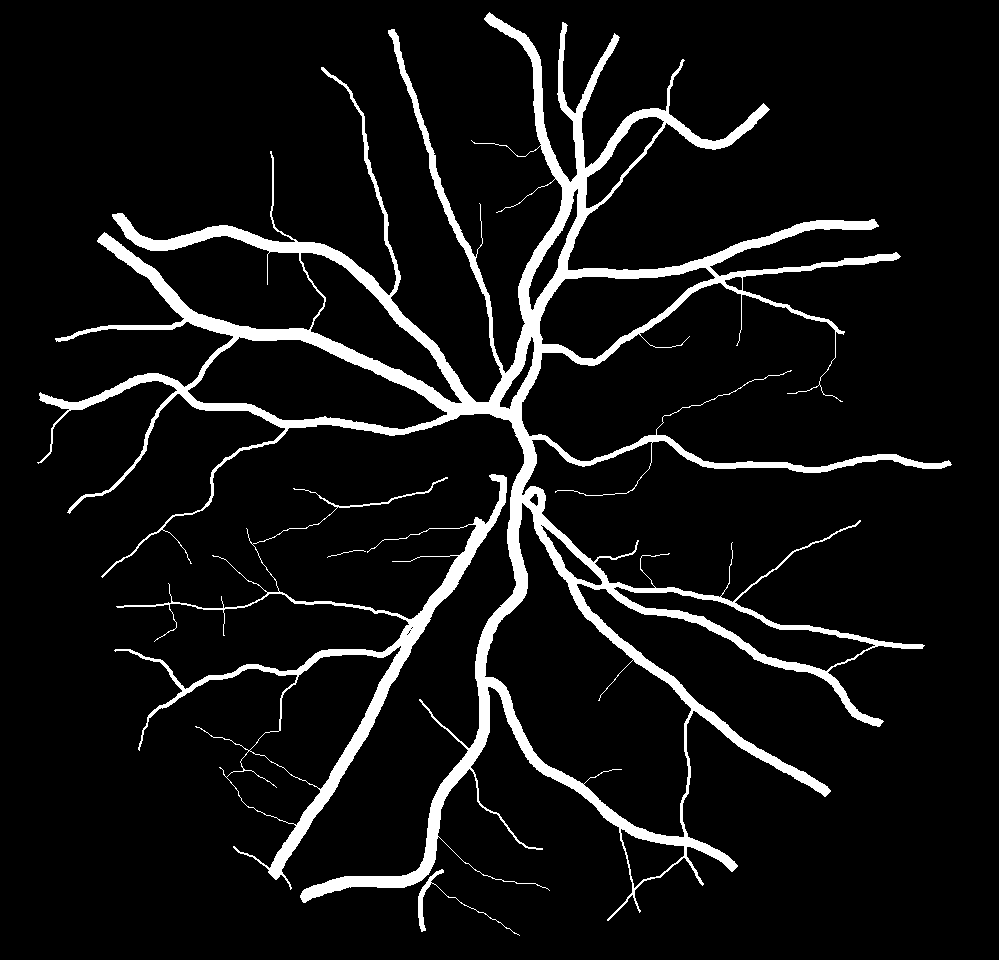
\includegraphics[width=\linewidth]{../chase/Image_07R_1stHO.png}
		\centering
			\small{maska ekspercka}
	\end{minipage}
\end{figure}
\input{./dane/przetwarzanie obrazu/07R.txt}
\input{./dane/uczenie maszynowe/07R.txt}
\input{./dane/głęboka sieć neuronowa/07R.txt}



		\subsection{Zdjęcie \textit{08L}}

\begin{figure}[!h]
	\centering
	\begin{minipage}{0.26\linewidth}
		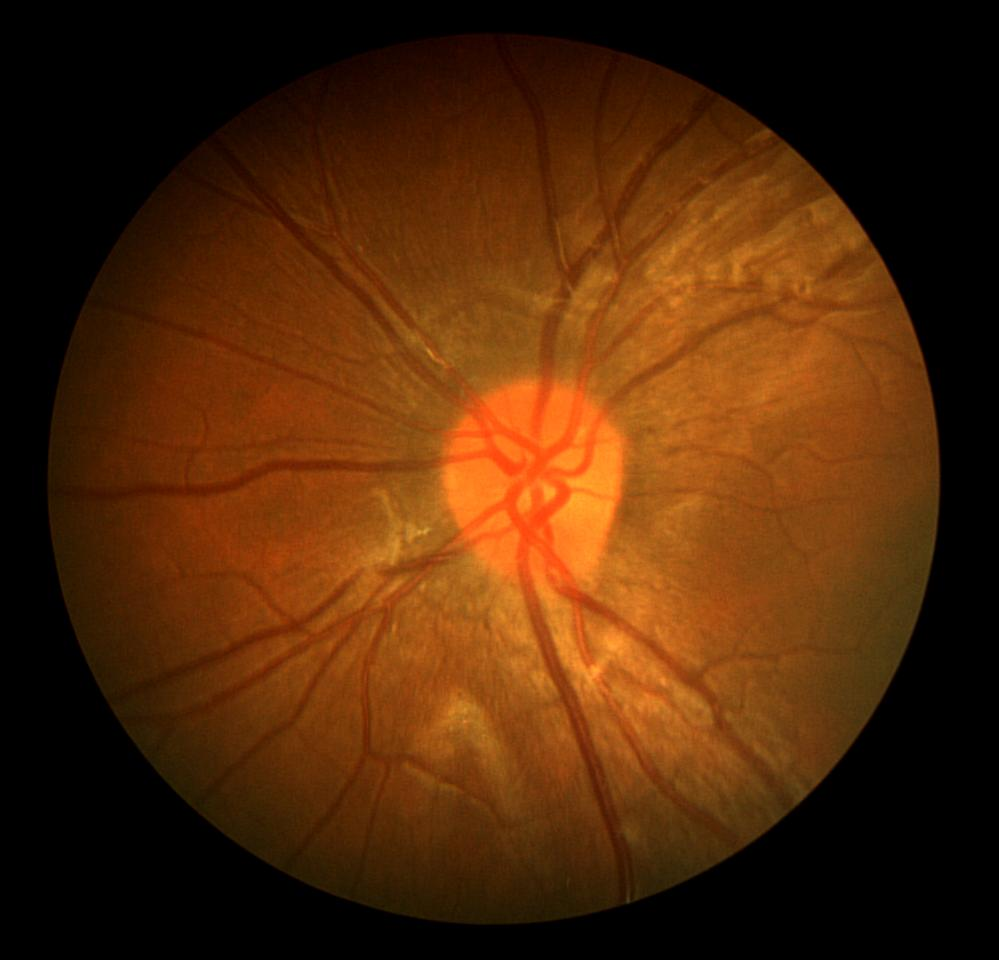
\includegraphics[width=\linewidth]{../chase/Image_08L.jpg}
		\centering
			\small{obraz wejściowy}
	\end{minipage}
	\hfill
	\begin{minipage}{0.26\linewidth}
		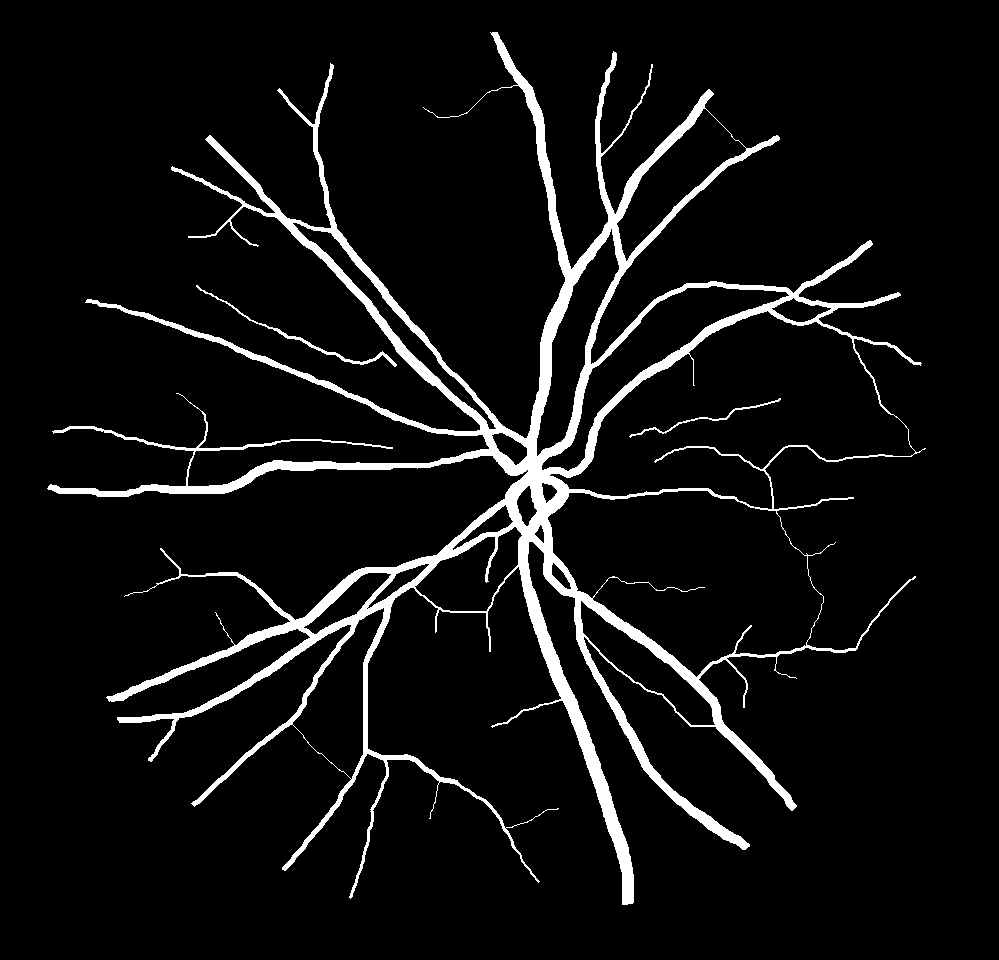
\includegraphics[width=\linewidth]{../chase/Image_08L_1stHO.png}
		\centering
			\small{maska ekspercka}
	\end{minipage}
\end{figure}
\input{./dane/przetwarzanie obrazu/08L.txt}
\input{./dane/uczenie maszynowe/08L.txt}
\input{./dane/głęboka sieć neuronowa/08L.txt}


	
	\section{Wnioski}
	
	 Przetwarzanie obrazu zwraca bardzo ograniczone wyniki,
	 ponieważ jest oparte na wykrywaniu krawędzi.
	 Ta metoda jest wrażliwa na szum oraz zmienną jasność na zdjęciu.
	 Najczęściej wynik końcowy to kompromis
	 pomiędzy brakiem wyników fałszywie pozytywnych, 
	 a wykryciem wszystkich naczyń.
	 
	 Metoda uczenia maszynowego, 
	 w porównaniu do zwykłego przetwarzania, 
	 lepiej wykrywa mniejsze naczynia.
	 W części przypadków liczba prawdziwie pozytywnych klasyfikacji jest większa w uczeniu maszynowym, 
	 a w części w zwykłym  przetwarzaniu obrazów.
	 Jest to spowodowane tym, 
	 że choć uczenie maszynowe lepiej wykrywa poszczególne naczynia (nawet te małe),
	 to w przypadku tych większych ma problemy z ich wypełnieniem.
	 Ta metoda ma największą liczbę przypadków fałszywie pozytywnych.
	 Powstały szum, można by zredukować, 
	 lecz utracilibyśmy również niektóre przypadki pozytywnego wykrycia naczyń.
	
	Sieć neuronowa całkiem dobrze radzi sobie z wykrywaniem naczyń.
	Dysponując większą mocą obliczeniową,
	można by zwiększyć liczbę warstw i uczyć na większych fragmentach obrazu,
	co poskutkowałoby jeszcze lepszym rezultatem.
	
	Podejścia różnią się czasem uzyskania rezultatu dla danego obrazu.
	W przypadku pierwszych dwóch podejść
	(i z wytrenowanym już klasyfikatorem) wynik można otrzymać
	w kilka sekund. W przypadku sieci neuronowej może to potrwać nawet kilka minut.
		
\end{document}